\chapter{The Problem} \label{ch:the-problem}

In this chapter, we will describe the problem addressed by EcoBeach, a system built as part of the Semester Project in Scalable Systems, on the first semester on the masters of Software Engineering SDU. \medbreak
\noindent
First, a problem definition will be given, along with the overall objective. Next, an in-depth problem description is presented, where the sub-problems will be unveiled, and why it is necessary to derive a solution.

\section{Problem and Objective}

At present, the ecology is threatened by increasing changes to the climate. One of the notable climate changes is the rising shorelines that are predicted to rise to critical heights in the 21st century. According to the publication, Sea level rise and its coastal impacts, by Anny Cazenave and Gonéri Le Cozannet, we will see an average increase of 40-75 cm on a global scale by the year 2100 \cite[p.~23]{sea-level-rise}. This increase will not happen uniformly, and some areas will see higher sea levels than others \cite[p.~21]{sea-level-rise}, which can result in sea level increases of up 30\% in some regions \cite[p.~23]{sea-level-rise}. In \autoref{fig:sea-level-rise} a projection of the expected sea-level rise by the year 2100 is illustrated.

\begin{figure}[h]
    \centering
    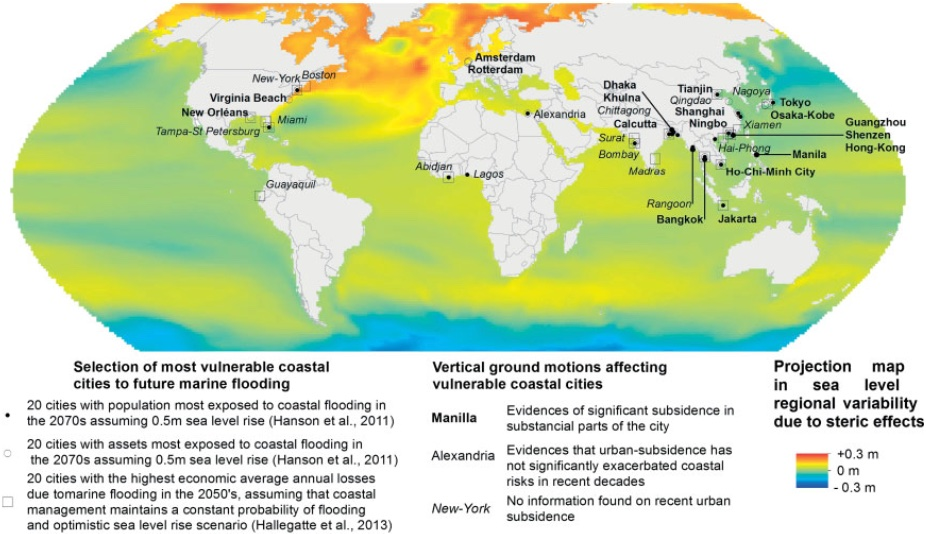
\includegraphics[width=\textwidth]{sea-level-rise.jpg}
    \caption{A projection of expected sea level regional variability by year 2100. Taken from, Sea level rise and its coastal impacts, by Anny Cazenave and Gonéri Le Cozannet \cite[p.~27]{sea-level-rise} (Copyrightable under the terms of \href{https://creativecommons.org/licenses/by-nc-nd/3.0/}{the Creative Commons Attribution-NonCommercial-NoDerivs License})}
    \label{fig:sea-level-rise}
\end{figure}

As rising shorelines are a growing threat, it is imperative to react and minimize climate change, but sadly, this might not be something humanity can do on time. Therefore, monitoring how the shorelines are changing is paramount to alleviate the risk of rising shorelines. This growing threat and the accompanying concerns preface the problem that is: \medbreak 
\noindent
\begin{quote}
    Humanity might not combat climate change to avoid massive floods in cities and countries. Currently, there are not enough accessible options to monitor how shorelines are changing to prepare for or predict floods. \medbreak 
\end{quote}

\noindent
This project aims to solve this problem by creating a system capable of processing satellite imagery of geo-locations worldwide in real-time to determine how the shorelines have changed and are changing. 

The project will rely on mobile sensing and various big data technologies and tools to create such a system.

\section{Problem Description} \label{sec:problem-description}

Monitoring shorelines is quite attractive; having historical and current data on shoreline changes can potentially help both the public and the private sector.  \medbreak 
\noindent
In the 21st century, governments will need to develop new and ingenious ways to combat the rising shorelines and avoid floods. Knowing where shorelines are rising the most can be a huge factor in helping decide where to preemptively build solutions that can help prevent large floodings and the destruction of properties and, potentially, cities.
Some governments already have needed to find solutions to flooding, which is apparent when looking at the Netherlands that have built resilient solutions to prevent floods, e.g., the Maeslantkering storm surge barrier \cite{maeslantkering}. 
\medbreak 
\noindent
It might also be beneficial to know how shorelines are changing in the private sector. Knowing this can be helpful to make informed decisions about where to settle down or prepare for floods for individuals living at places at risk.  \medbreak 
\noindent
From a technical perspective, creating a system capable of processing satellite imagery in real-time is a daunting task with many sub-problems that need to be solved to make it feasible.
To derive a solution, we believe the following sub-problems must be solved:

\begin{itemize}
    \item How to download satellite images from Copernicus?
    \item How to process images, so water is differentiated from land?
    \item How to build a system capable of handling big data? 
    \item How to build a system capable of real-time processing?
    \item How to build a highly resilient system?
    \item How to build a mobile application that uses mobile sensing in a meaningful way to visualize shoreline changes?
\end{itemize}
\noindent
It is paramount that these problems can be solved to derive a feasible solution to monitor shorelines in real-time. Such a solution, EcoBeach, is described in detail in the next chapter.
